\documentclass[]{article}
\usepackage{amsmath}
\usepackage{graphicx}
%\usepackage{xcolor}
\usepackage{hyperref}
\usepackage[dvipsnames]{xcolor}
\usepackage{matlab-prettifier}
\usepackage{array}
\usepackage{fullpage}

\graphicspath{ {images/} }
\usepackage{comment}

\setlength\parindent{0pt}

\title{Report: V{\small I}LMA}
\author{Jesus Miguel Adrian Matos}
\date{\today}


\begin{document}
\maketitle

\begin{abstract} 
This report is focused on explaining the \textbf{VILMA} funcionalities, we will not mention what datasets the \textbf{VILMA} tests ware made on, but rather we will explain how it selects the foil-caption to carry out the tests. Our report is structured as follows:

\textbf{Concepts section:} Concepts that are used in the report.

\textbf{Body section:} we list models that will be evaluated by VILMA and we explain the VILMA tests.

\textbf{Bonclusions section:} We observe several models on which the VILMA tests were applied, and we give a conclusion on VILMA benchmarks.




\end{abstract}

%\newpage 

\section{Previous concepts:}

\subsection{Image-Language models(IMLs):}
\noindent An image-language model is an artificial intelligence system designed to process and understand both visual and textual data, integrating these two modalities to perform various tasks. These models can generate text descriptions from images, produce images from text descriptions, and understand the relationships between visual and textual elements. Key capabilities and applications of image-language models include:

\begin{itemize}
\item \textbf{Image Captioning:} Generating descriptive text for a given image.
\item \textbf{Visual Question Answering (VQA):} Answering questions related to the content of an image.
\item \textbf{Image Generation from Text:} Creating images based on textual descriptions.
\item \textbf{Cross-modal Retrieval:} Finding images that match a given text or vice versa.
\item \textbf{Image-Text Matching:} Evaluating the relevance or similarity between an image and a text description.
\end{itemize}

\noindent These models typically combine techniques from computer vision (for processing videos) and natural language processing (for handling text). They often use deep learning architectures such as:

\begin{itemize}
\item \textbf{Convolutional Neural Networks (CNNs):} For extracting features from images.
\item \textbf{Transformers:} For handling and generating text, and sometimes for processing image features.
\item \textbf{Multimodal Models:} Like CLIP (Contrastive Language–Image Pretraining) and DALL-E, developed by OpenAI, which are specifically designed to understand and generate both images and text.
\end{itemize}
\subsection{Video-Language models(VidLMs):}
\noindent Video-language models are advanced machine learning systems designed to understand and generate both video content and associated natural language descriptions. These models can interpret and generate content involving the complex interplay between visual data (videos) and textual data (language). Key capabilities and applications of video-language models:

\begin{itemize}
\item \textbf{Video Captioning:} Automatically generating descriptive text for video content.
\item \textbf{Video Question Answering (Video QA):} Answering questions based on the content of a video.
\item \textbf{Text-to-Video Generation:} Creating video sequences from textual descriptions.
\item \textbf{Video Retrieval:} Finding relevant videos based on textual queries or descriptions.
\item \textbf{Action Recognition:} Identifying and classifying actions depicted in video clips.
\end{itemize}

\noindent These models typically combine techniques from computer vision (for processing videos) and natural language processing (for handling text). Here, there are some Architecture and Models:

\begin{itemize}
\item \textbf{Encoder-Decoder Frameworks:} Commonly used where the encoder processes video frames to create a rich representation and the decoder generates the corresponding textual description.
\item \textbf{Transformer-based Models:} These models leverage attention mechanisms to handle the complexity of video and language data, such as the Vision Transformer (ViT) and variants like VideoBERT.
\item \textbf{Fusion Techniques:} Methods to effectively combine and align visual and textual data, such as cross-modal attention and joint embedding spaces.
\end{itemize}
\section{Video Language Model Assessment(ViLMA):}

Es un benchmark independiente de la tarea que detalla evaluacion de las capacidades de los modelos(VidLMs) sobre una base firme.

Atravez de countrafactuales cuidadosamente selectionados, VILMA ofrece un conjunto de evaluciones controladas que arrojan luz sobre el verdadero potencial de estos modelos(VidLMs).

mientras tales evaluaciones arrojan luz sobre tareas de rendimiento y soporte para analisis coperativo, estos estan limitados a sus habilidades para revelar las capacidades visiolinguisticas que los modelos exiben a lo largo de las tareas.

\textbf{Comun estructura para cada test:}
\begin{enumerate}
\item In step 1, be harvested high-quality examples from existing \textbf{video-language datasets}.
\item In step 2, 
\end{enumerate}
\begin{thebibliography}{}
    
\bibitem{lei2021clipbert}
J. Lei et al., "Less is More: CLIPBERT for Video-and-Language Learning via Sparse Sampling," 2021 IEEE/CVF Conference on Computer Vision and Pattern Recognition (CVPR), Nashville, TN, USA, 2021, pp. 7327-7337, doi: 10.1109/CVPR46437.2021.00725.

\bibitem{Buchen-Mainardi 1975}
P.W. Buchen, F. Mainardi,Asymptotic expansions for transient viscoelastic waves, {\it Journal de M{\'e}canique} {14},  597--608 (1975).

\bibitem{AG-FM_MECC16}
A. Giusti, F. Mainardi, A dynamic viscoelastic analogy for fluid-filled elastic tubes, {\it Mecanica}, published on line, 04 February  2016.(2015).
\end{thebibliography}

\section{conclusion:}

In Figure \ref{fig:test_model} we can see the scores of the \textbf{VILMA} tests, for various models, where the letters \textbf{P} represent the main test and the \textbf{T} represents the \textbf{Proficiency test}.

These are ordered as follows, the first 2 are the \textbf{simple LM}, the next 2 are the \textbf{ILM}, and the rest are the \textbf{VidLM}.

\textbf{Observations from figure 2:}

So we can notice that the best scores are for the Image Language Model (ILM), the VidLMs have score aceptable, and as it was waiting, the LM are the ones with the lowest score, because they do not have images to validate some tests.

We can also noted that simple LMs have good scores in proficiency tests, since these do not imply a strong spatio-temporal relations.
\begin{figure}[h]
    \centering
    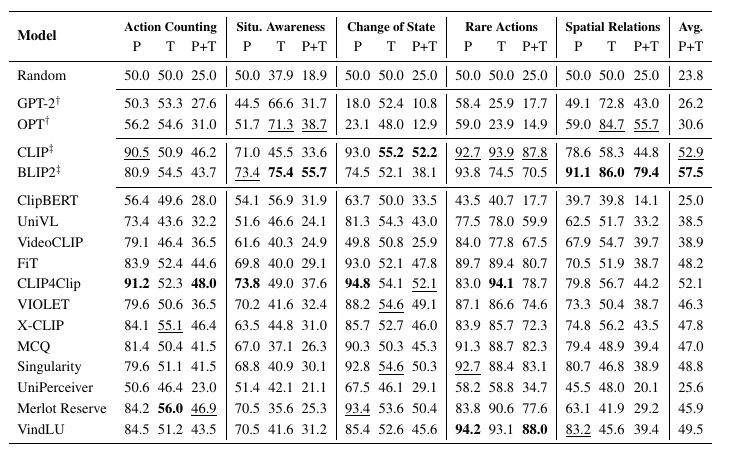
\includegraphics[width=0.25\textwidth]{test_model}
    \caption{Score of the models where the VILMA test was carried out}
    \label{fig:test_model}
\end{figure}

Therefore, I can conclud that VILMA is more focused on VidLM that has spatio-temporal relations for videos, and is also very good for ILM, since the frames of a video are images and VILMA uses a constant frequency of frames to carry out their tests, which allows us to have images that represent periods of frames, and with this method a video could be considered as a set of images but with a space-time relations.

\end{document}          
